\documentclass{ieeeojies}
\usepackage{cite}
\usepackage{amsmath,amssymb,amsfonts}
\usepackage{algorithmic}
\usepackage{graphicx}
\usepackage{textcomp}
\usepackage{array}
\usepackage[table]{xcolor}
\usepackage{multirow}
\usepackage{multicol}
\usepackage{float}
\usepackage{hyperref}

\def\BibTeX{{\rm B\kern-.05em{\sc i\kern-.025em b}\kern-.08em
    T\kern-.1667em\lower.7ex\hbox{E}\kern-.125emX}}

\begin{document}
\title{PREDICTING THREE CRYPTOCURRENCY PRICES USING TIME SERIES APPROACH}

\author
{\uppercase{TRINH DUC}\authorrefmark{1},
\uppercase{TRUONG MINH DUC}\authorrefmark{2},
\uppercase {DO PHUONG NGHI}\authorrefmark{3}
\uppercase and {PHAM CAO NGUYEN}\authorrefmark{4}}

\address[1]{Faculty of Information Systems, University of Information Technology, (e-mail: 21521969@gm.uit.edu.vn)}
\address[2]{Faculty of Information Systems, University of Information Technology, (e-mail: 21521971@gm.uit.edu.vn)}
\address[3]{Faculty of Information Systems, University of Information Technology, (e-mail: 21522372@gm.uit.edu.vn)}
\address[3]{Faculty of Information Systems, University of Information Technology, (e-mail: 21522395@gm.uit.edu.vn)}

\begin{abstract}
The volatility and unpredictability of cryptocurrency markets pose significant challenges for investors and analysts alike. In this paper, we explore the application of time series analysis techniques to predict cryptocurrency prices. With a focus on three major cryptocurrencies: ETH/USDT, BNB/USDT and BTC/USDT, we apply Linear Regresstion (LR), ARIMA, RNN, GRU, LSTM, Holt-Winters, SES, ResCNN models to predict cryptocurrency prices. In addition, we utilize three evaluation metrics MAE, MAPE, RMSE and WAPE to assess the performance of models and identify which ones yield the best results. We also employ the Adam optimization algorithm to enhance the training efficiency and convergence speed of our predictive models, thereby optimizing the accuracy of cryptocurrency price forecasts across various time series analysis techniques.
\end{abstract}

\begin{keywords}
Cryptocurrency, prediction, time series analysis
\end{keywords}

\titlepgskip=-15pt

\maketitle

\section{Introduction}
\label{sec:introduction}
Cryptocurrency, a revolutionary digital asset class, has gained significant attention since the emergence of Bitcoin (BTC) in 2009, challenging traditional notions of currency and investment. The main challenge is predicting the future prices of cryptocurrencies like Ethereum (ETH/USDT), Binance Coin (BNB/USDT) and Bitcoin (BTC/USDT) due to their volatile and complex market nature.\\
Accurate forecasting offers substantial opportunities for investors and analysts, including increasing revenue through timely buy/sell decisions, attracting more users to trading platforms with valuable predictions, and potentially driving up Bitcoin's price through informed investment strategies.\\
This report explores time series analysis techniques on historical price data from the past 24 hours to predict prices for the next 24 hours, utilizing models such as Linear Regresstion (LR), Autoregressive Integrated Moving Average (ARIMA), Recurrent Neural Network (RNN), Gated Recurrent Unit (GRU), Long Short-Term Memory (LSTM), Holt-Winters, Simple Exponential Smoothing (SES) and ResCNN. By leveraging these models, the study aims to provide insights for navigating the dynamic cryptocurrency markets. Evaluation metrics like Mean Absolute Error (MAE), Mean Absolute Percentage Error (MAPE), Root Mean Square Error (RMSE), and Weighted Absolute Percentage Error (WAPE) are used to compare model performance and identify the most suitable approach for reliable predictions.

\section{Related Works}
Predicting cryptocurrency prices has garnered considerable attention due to the market's high volatility and potential for significant financial gains. Various methodologies have been explored, ranging from traditional statistical models to sophisticated machine learning and deep learning techniques.\\
Traditional time series models, such as Linear Regression (LR) and Autoregressive Integrated Moving Average (ARIMA), have been foundational in time series financial forecasting. Linear Regression models have been employed to establish baseline predictions by capturing linear relationships in historical price data. ARIMA, known for its ability to handle non-stationary data and its capacity to model linear temporal dependencies in financial time series data. However, in “Automated Bitcoin trading via machine learning algorithms” \cite{b1}, the authors compare various machine learning models for cryptocurrency price prediction and note the limitations of ARIMA models in capturing the highly volatile nature of Bitcoin prices. Studies also shown that while ARIMA can effectively model linear trends and seasonality, its performance diminishes with highly volatile and non-linear data typical of cryptocurrency markets.\\
Exponential smoothing methods, including Holt-Winters and Simple Exponential Smoothing (SES), have also popular for time series forecasting. These methods are effective for data with clear trends and seasonal components. The Holt-Winters method is known for its triple exponential smoothing capability, can model seasonality effectively. While SES provides a smoothed representation of the data. "On Forecasting Cryptocurrency Prices: A Comparison of Machine Learning, Deep Learning, and Ensembles" \cite{b2} point out the limitations of traditional methods like Holt-Winters and Simple Exponential Smoothing, stating that these methods often fall short in capturing the erratic and non-linear nature of cryptocurrency price movements.\\
Recurrent Neural Networks (RNN), Gated Recurrent Units (GRU), and Long Short-Term Memory (LSTM) networks, these machine learning models are designed to handle sequential data and have shown superior performance in predicting time series data by leveraging their ability to remember long-term dependencies, offering improvements over traditional models by capturing complex, non-linear relationships. LSTM networks, in particular, have been widely adopted due to their capacity to mitigate the vanishing gradient problem, which is common in RNNs. Rushil Yavasani and Frank Wang, through “Comparative Analysis of LSTM, GRU, and ARIMA Models for Stock Market Price Prediction” \cite{b3}, emphasizes that LSTM and GRU models are better at handle long-term dependencies and non-linear patterns compared to traditional methods with a outperform results.\\

\section{Materials}
\subsection{Dataset}
The data for this study originates from https://www.gate.io/vi, a prominent cryptocurrency exchange known for its extensive range of tokens, attracting a significant user base within the investor community. It comprises information on three major cryptocurrencies: Ethereum (ETH/USDT), Binance Coin (BNB/USDT) and Bitcoin (BTC/USDT).\\
Utilizing this dataset ensures the credibility of our analysis. Spanning from January 1, 2021, to February 29, 2024, the dataset offers a comprehensive temporal coverage essential for our research.\\
K-line data is generated according to transaction data, so data is only available at the time a transaction occurs, data is not available at this time when there is no transaction. K-line includes the following time units: 30s, 1m, 5m, 1h, 4h, 1d, 7d and a file will be created for each trading pair per month . For K-line 30s, 1m, 5m, 1h , 4h and 1d, the previous month's data file will be created on the 1st of every month.\\
    \indent\ Timestamp (TS): Timestamp, in seconds\\
    \indent\ Volume (V): Transaction volume\\ 
    \indent\ Close (C): Close price\\
    \indent\ High (H): Highest price\\ 
    \indent\ Low (L): Lowest price\\
    \indent\ Open (O): Open price\\

\subsection{Tools}

During our research, we utilized various statistical analysis tools in Python such as numpy, pandas, sklearn, matplotlib.pyplot, to better understand data patterns and draw meaningful conclusions. These tools facilitated a deeper comprehension of the data, resulting in significant findings presented in accompanying tables and charts.

\subsection{Descriptive Statistics}
\begin{table}[H]
  \centering
  \caption{Descriptive statistics of BNB}
\begin{tabular}{|>{\columncolor{red!20}}c|c|c|c|}
    \hline
    \rowcolor{red!20} & ETH & BNB & BTC \\ \hline
    Mean & 2202.092342 & 322.9943283 & 35373.61203 \\ \hline 
    Standard Error & 5.092162066 & 0.692032333 & 75.20108046 \\ \hline
    Median & 1892.37 & 305.0411 & 34008.005 \\ \hline
    Mode & 1816.53 & 233.5 & 16966.7 \\ \hline
    Standard Deviation & 847.4434797 & 115.1688184 & 12515.05048 \\ \hline 
    Sample Variance & 718160.4513 & 13263.85672 & 156626488.5 \\ \hline
    Kurtosis & 0.267036293 & 1.012787554 & -0.757466742 \\ \hline
    Skewness & 1.002497998 & 0.548524786 & 0.414513702 \\ \hline
    Range & 4128.1 & 648.7428 & 52971.2 \\ \hline
    Minimum & 719.99 & 35.7463 & 15649.7 \\ \hline
    Maximum & 4848.09 & 684.4891 & 68620.9 \\ \hline
    Sum & 60989149.5 & 8945650.917 & 979707558.8 \\ \hline
    Count & 27696 & 27696 & 27696 \\ \hline
\end{tabular}
\end{table}

\begin{figure}[H]
    \centering
    \begin{minipage}{0.23\textwidth}
    \centering
    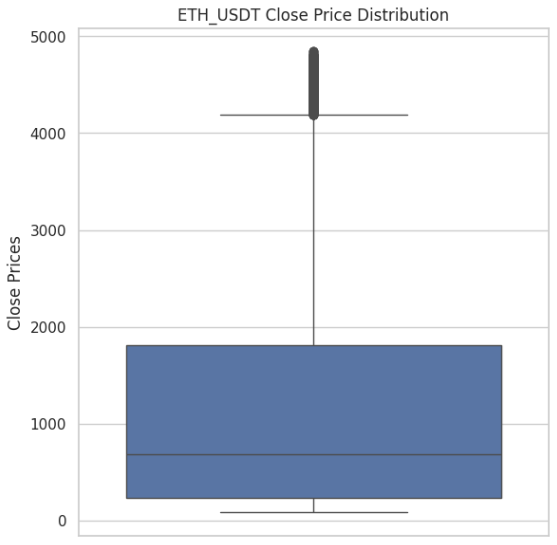
\includegraphics[width=1\textwidth]{bibliography/ETH_box.png}
    \caption{ETH/USDT's close price boxplot}
    \label{fig:enter-label}
    \end{minipage}
    \hfill
    \begin{minipage}{0.23\textwidth}
    \centering
    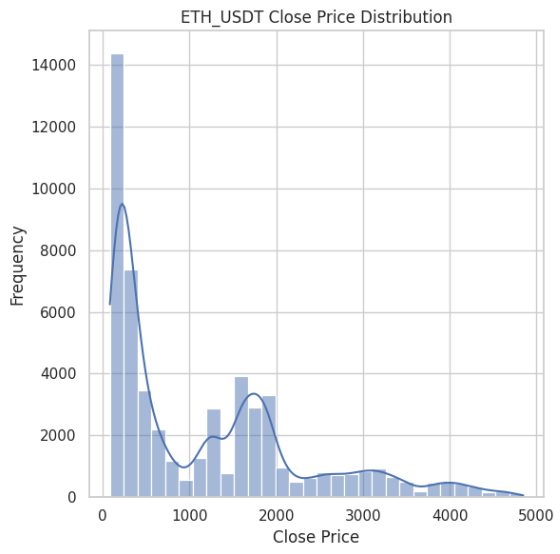
\includegraphics[width=1\textwidth]{bibliography/ETH_hist.png}
    \caption{ETH/USDT's close price histogram}
    \label{fig:enter-label}
    \end{minipage}
    \hfill
    \begin{minipage}{0.23\textwidth}
    \centering
    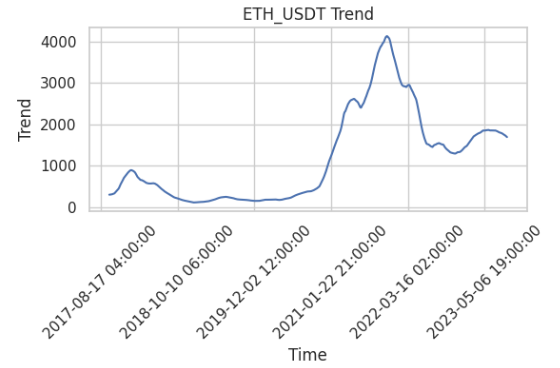
\includegraphics[width=1\textwidth]{bibliography/ETH_trend.png}
    \caption{ETH/USDT's trend}
    \label{fig:enter-label}
    \end{minipage}
    \hfill
    \begin{minipage}{0.23\textwidth}
    \centering
    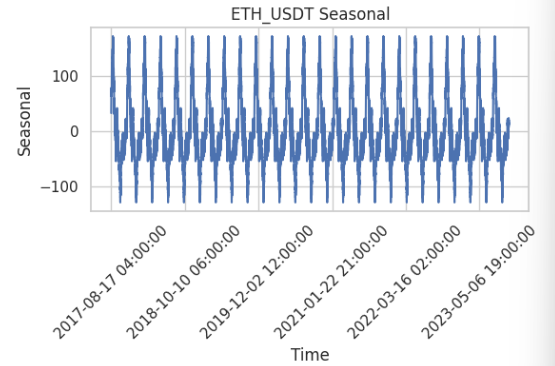
\includegraphics[width=1\textwidth]{bibliography/ETH_seasonal.png}
    \caption{ETH/USDT's seasonal}
    \label{fig:enter-label}
    \end{minipage}
\end{figure}

\begin{figure}[H]
    \centering
    \begin{minipage}{0.23\textwidth}
    \centering
    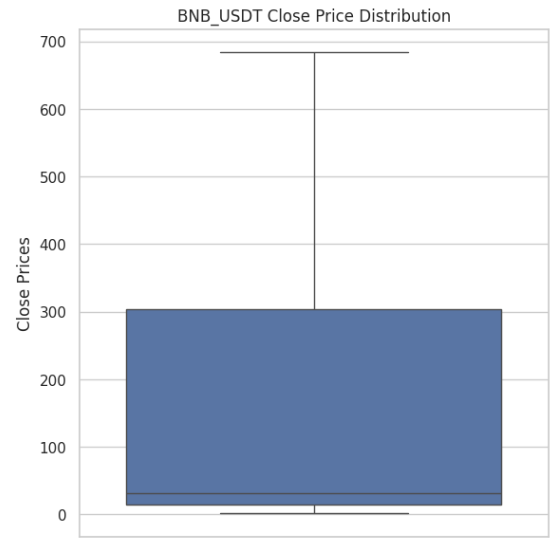
\includegraphics[width=1\textwidth]{bibliography/BNB_box.png}
    \caption{BNB/USDT's close price boxplot}
    \label{fig:enter-label}
    \end{minipage}
    \hfill
    \begin{minipage}{0.23\textwidth}
    \centering
    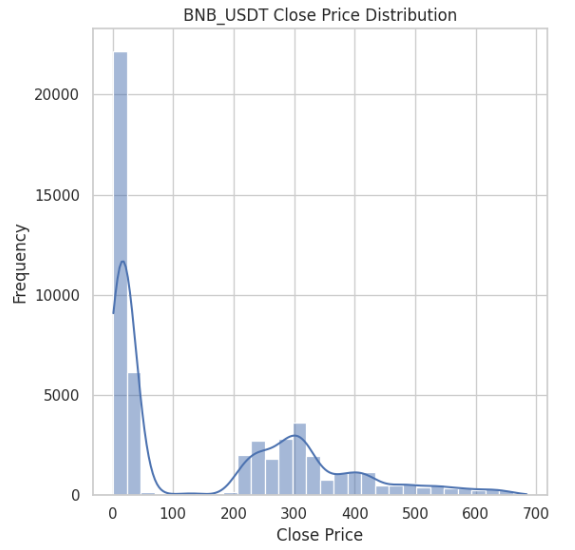
\includegraphics[width=1\textwidth]{bibliography/BNB_hist.png}
    \caption{BNB/USDT's close price histogram}
    \label{fig:enter-label}
    \end{minipage}
\end{figure}

\begin{figure}[H]
    \centering
    \begin{minipage}{0.23\textwidth}
    \centering
    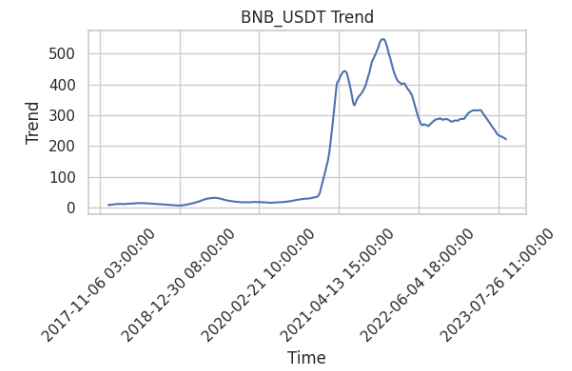
\includegraphics[width=1\textwidth]{bibliography/BNB_trend.png}
    \caption{BNB/USDT's trend}
    \label{fig:enter-label}
    \end{minipage}
    \hfill
    \begin{minipage}{0.23\textwidth}
    \centering
    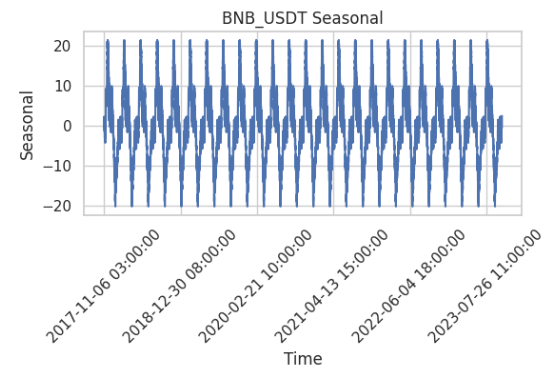
\includegraphics[width=1\textwidth]{bibliography/BNB_seasonal.png}
    \caption{BNB/USDT's seasonal}
    \label{fig:enter-label}
    \end{minipage}
\end{figure}

\begin{figure}[H]
    \centering
    \begin{minipage}{0.23\textwidth}
    \centering
    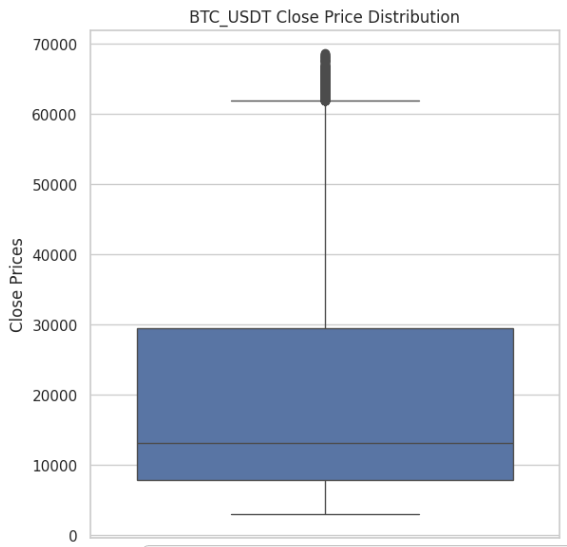
\includegraphics[width=1\textwidth]{bibliography/BTC_box.png}
    \caption{BTC/USDT's close price boxplot}
    \label{fig:enter-label}
    \end{minipage}
    \hfill
    \begin{minipage}{0.23\textwidth}
    \centering
    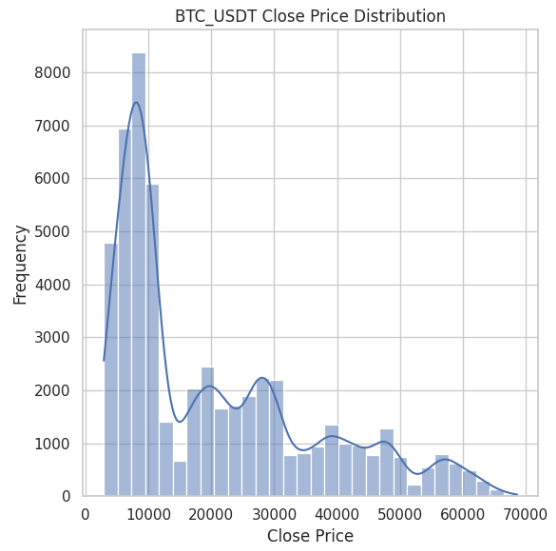
\includegraphics[width=1\textwidth]{bibliography/BTC_hist.png}
    \caption{BTC/USDT's close price histogram}
    \label{fig:enter-label}
    \end{minipage}
    \hfill
    \begin{minipage}{0.23\textwidth}
    \centering
    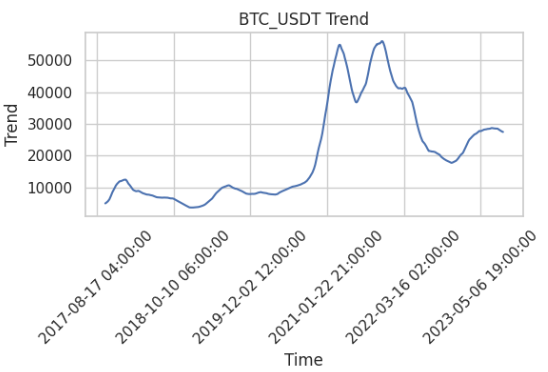
\includegraphics[width=1\textwidth]{bibliography/BTC_trend.png}
    \caption{BTC/USDT's trend}
    \label{fig:enter-label}
    \end{minipage}
    \hfill
    \begin{minipage}{0.23\textwidth}
    \centering
    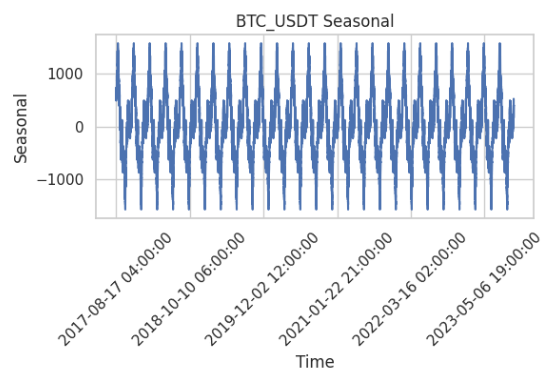
\includegraphics[width=1\textwidth]{bibliography/BTC_seasonal.png}
    \caption{BTC/USDT's seasonal}
    \label{fig:enter-label}
    \end{minipage}
\end{figure}

\section{Methodology}
\subsection{Linear Regression}
Regression analysis is a tool for building mathematical and statistical models that characterize relationships between a dependent variable and one or more independent, or explanatory, variables, all of which are numerical. This statistical technique is used to find an equation that best predicts the y variable as a linear function of the x variables.\\
A multiple linear regression model has the form: 
\[Y=\beta_0+\beta_1X_1+\beta_2X_2+\cdots+\beta_kX_k+\varepsilon\]
\\
Where:\\
	\indent\ Y is the dependent variable (Target Variable).\\
	\indent\ \(X_1, X_2, \ldots, X_k\) are the independent (explanatory) variables.\\
	\indent\ \(\beta_0\) is the intercept term.\\
	\indent\ \(\beta_1,..., \beta_k\) are the regression coefficients for the independent variables.\\
	\indent\ \(\varepsilon\) is the error term.

\subsection{ARIMA}
ARIMA \cite{b4} is a popular and powerful time series forecasting method. It is used to model the relationship between a time series and its lagged values, as well as its past errors or residuals.\\
ARIMA are widely used in various fields such as finance, economics, and meteorology for forecasting purposes. They can capture both the trend and seasonality in time series data, making them versatile for a wide range of forecasting tasks.\\

The ARIMA is defined by three main components:\\
	\indent\textbullet\ Autoregression (AR): captures the relationship between the current observation and its lagged (past) observations. It models the dependence of the current value on its own past values.
	\[ Y_t = \phi_0 + \phi_1 Y_{t-1} + \phi_2 Y_{t-2} + \cdots + \phi_p Y_{t-p} \]
	\indent\textbullet\ Moving Average (MA): models the relationship between the current observation and a linear combination of past errors (residuals) from a moving average model.
	\[ Y_t = \mu + \theta_1 \varepsilon_{t-1} + \theta_2 \varepsilon_{t-2} + \cdots + \theta_q \varepsilon_{t-q} + \varepsilon_t \]
	\indent\textbullet\ Differencing (I): refers to the differencing operation applied to the time series data to make it stationary, i.e., removing trends and seasonality. It involves taking the difference between consecutive observations.\\
 
The ARIMA model is denoted by the notation ARIMA(p, d, q), where:\\
    \indent\textbullet\ p: The order of the autoregressive (AR) component, representing the number of lagged observations included in the model.\\
    \indent\textbullet\ d: The degree of differencing required to make the time series stationary.\\
    \indent\textbullet\ q: The order of the moving average (MA) component, representing the number of lagged forecast errors included in the model.\\
    
The general formula for an ARIMA(p, d, q) model:
    \[ Y_t = \mu + \phi_1 Y_{t-1} + \cdots + \phi_p Y_{t-p} + \theta_1 \varepsilon_{t-1} + \cdots + \theta_q \varepsilon_{t-q} + \varepsilon_t \]

The ARIMA model also involves a differencing (I) step to make the time series stationary. This is represented by taking the difference between consecutive observations:
    \[ Y'_t = Y_t - Y_{t-1} \]
\\
Where:\\
    \indent\ \(t\) is a specific point in time.\\
    \indent\ \(c\) is a constant value.\\
    \indent\ \(Y_t\) is the value of the time series at time t.\\
    \indent\ \(Y'_t\) is the value of the differenced series at time t.\\
    \indent\ \( Y_{t-1}, Y_{t-2}, \cdots, Y_{t-p} \) are lagged values of the time series.\\
    \indent\ \( \phi_1, \phi_2, \cdots, \phi_p \) are the autoregressive (AR) coefficients.\\
    \indent\ \( \varepsilon_{t-1}, \varepsilon_{t-2}, \cdots, \varepsilon_{t-p} \) are the moving average (MA) coefficients.\\
    \indent\ \( \varepsilon_t \) is the error term at time t.

\subsection{RNN}
RNN \cite{b5} is a type of artificial neural network designed to process sequential data. The architecture of an RNN consists of repeating units or cells, each of which has a connection to itself from the previous time step.\\

\begin{figure}[H]
    \centering
    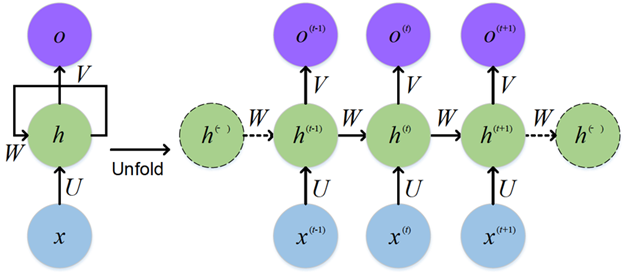
\includegraphics[width=\linewidth]{bibliography/RNN.png}
    \caption{Recurrent Neural Network Architecture} \cite{b6}
    \label{fig:enter-label}
\end{figure}
    
RNN are commonly used in tasks such as natural language processing (NLP), speech recognition, time series analysis, and many others where the input data has a sequential nature.\\

\textbf{Formulas}\\
The formula for calculating the current state:
    \[h_t = f(h_{t-1}, x_t)\]
The formula for applying Activation function (tanh):
    \[h_t = \tanh(W_{hh} h_{t-1} + W_{xh} x_t)\]
The formula for calculating output:
    \[y_t = W_{hy} h_t\]
\\
Where:\\
    \indent\ \(h_t\) is the hidden state at time t (current state).\\
    \indent\ \(h_(t-1)\) is the hidden state at time t-1 (previous state).\\
    \indent\ \(x_t\) is the input state at time t.\\
    \indent\ \(y_t\) is the output state at time t.\\
    \indent\ \(W_hx\) is the weight matrix connecting the input \(x_t\) to the hidden state \(h_t\).\\
    \indent\ \(W_hh\) is the weight matrix connecting the previous hidden state \(h_(t-1)\) to the current hidden state \(h_t\).\\
    \indent\ \(W_hy\) is the weight matrix connecting the hidden state \(h_t\) to the output \(y_t\).\\
    \indent\ \(f\) is the activation function applied to the hidden state, often a non-linear function such as tanh or ReLU.

\subsection{GRU}
GRU \cite{b7} is a variant of the standard Recurrent Neural Network (RNN). GRU is designed to address the issue of training traditional RNNs on long sequences, which often leads to the vanishing gradient problem.\\
The mechanism of GRU includes an update gate and a special reset gate, which help control the flow of information and adjust the "forgetting" of unnecessary information from the past. Specifically, at each time step, GRU receives input from the previous timestep and the current hidden state. It uses the update gate to decide whether new information should be updated from the current input, and uses the special gate to determine which information from the past should be "forgotten" or "remembered" to update the new hidden state.\\
\\
Update gate:
    \[z_t = \sigma(W_z \times [h_{t-1}, x_t] + b_z)\]
Reset gate:
    \[r_t = \sigma\left(W_r \times \left[ h_{t-1}, x_t \right] + b_r \right)\]
Candidate activation:
    \[\tilde{h}_t = \tanh(W_h \times [r_t \odot h_{t-1}, x_t] + b_h)\]
Hidden state update:
    \[h_t = (1 - z_t) \odot h_{t-1} + z_t \odot \tilde{h}_t\]
\\
Where:\\
    \indent\ \(\sigma\) is the sigmoid activation function.\\
    \indent\ \(\odot\) is element-wise multiplication \(((A \odot B)_{ij} = (A)_{ij} \times (B)_{ij})\).\\
    \indent\ \(x_t\) is the input at time t.\\
    \indent\ \(h_t\) is the hidden state at time \(t\) (current state).\\
    \indent\ \(h_{t-1}\) is the hidden state at time \(t-1\) (previous state).\\
    \indent\ \([h_{t-1}, x_t]\) denotes the concatenation of the previous hidden state \(h_{t-1}\) and the current input \(x_t\).\\
    \indent\ \(W_z, W_r, W_h\) are weight matrices for the update gate, reset gate, and candidate activation..\\
    \indent\ \(b_z, b_r, b_h\) are bias terms.

\subsection{LSTM}
LSTM \cite{b8} is a variant of the standard Recurrent Neural Network (RNN). LSTM is designed to address the problem of training RNNs on long sequences, particularly the issue of vanishing gradients.\\
LSTMs use a cell state to store information about past inputs. This cell state is updated at each step of the network, and the network uses it to make predictions about the current input. The cell state is updated using a series of gates that control how much information is allowed to flow into and out of the cell.\\
Specifically, each LSTM cell consists of the following gates:\\
    \indent\textbullet\ Forget Gate: determines which information in the previous state should be discarded.\\
    \indent\textbullet\ Input Gate: determines which new information should be added to the hidden state.\\
    \indent\textbullet\ Output Gate: determines which information in the hidden state should be outputted.\\
\\
Forget gate:
    \[f_t = \sigma(W_f \cdot [h_{t-1}, x_t] + b_f)\]
Input gate:
    \[i_t = \sigma(W_i \cdot [h_{t-1}, x_t] + b_i)\]
Candidate cell state:
    \[\tilde{c}_t = \tanh(W_c \cdot [h_{t-1}, x_t] + b_c)\]
New cell state:
    \[c_t = f_t \odot c_{t-1} + i_t \odot \tilde{c}_t\]
Output gate:
    \[o_t = \sigma(W_o \cdot [h_{t-1}, x_t] + b_o)\]
Hidden state:
    \[h_t = o_t \odot \tanh(c_t)\]
\\
Where:\\
    \indent\ \(\sigma\) is the sigmoid activation function.\\
    \indent\ \(\odot\) is element-wise multiplication \(((A \odot B)_{ij} = (A)_{ij} \times (B)_{ij})\).\\
    \indent\ \(x_t\) is the input at time t.\\
    \indent\ \(h_t\) is the hidden state at time \(t\) (current state).\\
    \indent\ \(h_{t-1}\) is the hidden state at time \(t-1\) (previous state).\\
    \indent\ \([h_{t-1}, x_t]\) denotes the concatenation of the previous hidden state \(h_{t-1}\) and the current input \(x_t\).\\
    \indent\ \(W_f, W_i, W_c, W_o\) are weight matrices for the forget gate, input gate, candidate cell gate, and output gate.\\
    \indent\ \(b_f, b_i, b_c, b_o\) are bias terms.

\subsection{Holt - Winters}
The Holt-Winters \cite{b9} method is a forecasting technique used to predict future values in time series data. The Holt-Winters method comprises three main components:\\
    \indent\textbullet\ Level (Average) (Overall): represents the average value of the series over time, indicates the baseline or the long-term average behavior of the data.\\
    \indent\textbullet\ Trend (Slope): accounts for the direction and rate of change in the data over time. It allows the method to capture increasing or decreasing trends in the series.\\
    \indent\textbullet\ Seasonality: refers to repeating patterns or cycles within the data that occur at fixed intervals, such as daily, weekly, or yearly patterns.\\

\textbf{Holt-Winters’ additive method:}\\
Level Equation: 
    \[L_t = \alpha(Y_t - S_{t-n}) + (1 - \alpha)(L_{t-1} + T_{t-1})\]
Trend Equation: 
    \[T_t = \beta(L_t - L_{t-1}) + (1 - \beta) T_{t-1}\]
Seasonal Equation:
    \[S_t = \gamma(Y_t - L_t) + (1 - \gamma) S_{t-n}\]
Forecast Equation:
    \[F_{t+h} = L_t + h \cdot T_t + S_{t+h-n(k+1)}\]

\textbf{Holt-Winters’ multiplicative method:}\\
Level Equation:
    \[L_t = \alpha \frac{Y_t}{S_{t-n}} + (1 - \alpha)(L_{t-1} + T_{t-1})\]
Trend Equation:
    \[T_t = \beta (L_t - L_{t-1}) + (1 - \beta) T_{t-1}\]
Seasonal Equation:
    \[S_t = \gamma \frac{Y_t}{L_t} + (1 - \gamma) S_{t-n}\]
Forecast Equation:
    \[F_{t+h} = (L_t + h \cdot T_t) S_{t+h-n(k+1)}\]
\\
Where:\\
    \indent\ \(t\) is a specific point in time.\\
    \indent\ \(n\) is the length of the seasonal cycle (i.e. n is the number of seasons in a year).\\
    \indent\ \(k\) is the integer part of \(\frac{h-1}{n}\), which ensures that the estimates of the seasonal indices used for forecasting come from the final year of the sample.\\
    \indent\ \(\alpha, \beta, \gamma\) Smoothing parameters for the level, trend, and seasonal components (\(0 \leq \alpha, \beta, \gamma \leq 1\)). \\
    \indent\ \(Y_t\) is the observed value at time \(t\).\\
    \indent\ \(L_t\) is the level component at time t.\\
    \indent\ \(T_t\) is the trend component at time t.\\
    \indent\ \(S_t\) is the seasonal component at time t.\\
    \indent\ \(F_{t+h}\) is the forecasted value at time \(t+h\).

\subsection{SES}
Simple Exponential Smoothing (SES) \cite{b9} is a basic and widely used method for forecasting time series data. It's a univariate time series forecasting technique that is easy to understand and implement. This method is suitable for forecasting data with no clear trend or seasonal pattern.\\
In SES, the forecast for the next time period is based solely on the weighted average of past observations. The basic principle is to assign exponentially decreasing weights to past observations, with more recent observations receiving higher weights.\\
The formula for Simple Exponential Smoothing is as follows:
    \[F_{t+1} = \alpha Y_t + (1 - \alpha) F_t\]
Where:\\
    \indent\ \(t\) is a specific point in time.\\
    \indent\ \(\alpha\) is the smoothing parameter (\(0 \leq \alpha \leq 1\)).\\
    \indent\ \(F_{t+1}\) is the forecasted value at the next time period \(t+1\).\\
    \indent\ \(Y_t\) is the observed value at time t.\\
    \indent\ \(F_t\) is the forecasted value at the current time period t.

\subsection{ResCNN}
Residual Convolutional Neural Network (ResCNN \cite{b10} is a neural network architecture used in deep learning, especially for computer vision tasks. It enhances traditional CNNs by adding residual connections, which allow the network to learn residual mappings. These connections bypass one or more convolutional layers, combining their outputs with the original input to help address the vanishing gradient problem. This enables effective training of very deep networks. ResCNNs typically include multiple convolutional layers with activation functions like ReLU, followed by residual connections, making them highly effective for tasks like image classification, object detection, and image segmentation.\\

\begin{figure}[H]
    \centering
    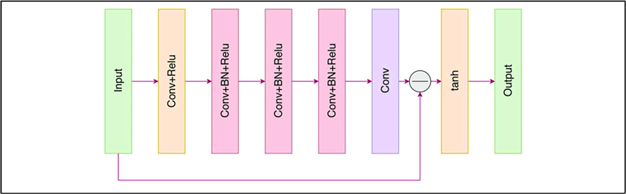
\includegraphics[width=\linewidth]{bibliography/ResCNN.png}
    \caption{The architecture of the proposed ResCNN network}
    \label{fig:enter-label}
\end{figure}

\textbf{Operation:}\\
In a typical convolutional neural network (CNN), each layer's output is passed through an activation function and then forwarded to the next layer. In a ResCNN, residual connections are introduced, which skip one or more layers and add the output of an earlier layer to a later layer.\\
Let's denote the input to a layer as X, and the output of that layer as \(F(X)\). The residual connection can be represented as:\\
    \[Output=F(X)+X\]
This allows the network to learn the residual mapping, or the difference between the input and output, instead of the full mapping. This approach helps in training deeper networks more effectively by addressing the vanishing gradient problem. A ResCNN stacks convolutional layers with these residual connections, often including pooling layers and activation functions. The specific architecture depends on the problem being solved.\\

\section{Result}
\subsection{Evaluation Methods}
\textbf{Mean Absolute Error} (MAE) \cite{b11}: is a metric used to evaluate the average absolute difference between predicted values and actual values.\\
    \[MAE = \frac{1}{n} \sum_{i=1}^{n} |y_i - \hat{y}_i|\]
\textbf{Mean Absolute Percentage Error} (MAPE) \cite{b11}: is the average percentage error in a set of predicted values.\\
    \[MAPE=\frac{100\%}{n}  \sum_{i=1}^{n} |y_i-\hat{y_i} |  = 1 \]
\textbf{Root Mean Squared Error} (RMSE) \cite{b11}: is the square root of average value of squared error in a set of predicted values.\\
    \[RMSE=\sqrt{\sum_{i=1}^{n} \frac{(\hat{y_i}-y_i )^2}{n} }\]
\textbf{Weighted Absolute Percentage Error} (WAPE) \cite{b11}: measures the weighted average of absolute percentage errors between predicted and actual values.\\
    \[WAPE = \frac{1}{\sum_{i=1}^{n} w_i} \sum_{i=1}^{n} w_i \left| \frac{y_i - \hat{y}_i}{y_i} \right| \times 100\%\]
Where: \\
    \indent\ \(N\) is number of time series (number of items) in the dataset.\\
    \indent\ \(H\) is length of the forecast horizon (prediction\_length).\\
    \indent\ \(T\) is length of the observed time series.\\
    \indent\ \(y_(i,t)\) is observed value of time series i at time t.\\
    \indent\ \(f_{i,t}\) is observed value of time series i at time t.\\
    \indent\ \(t\) is a specific point in time.\\
    \indent\ \(n\) is the number of data points.\\
    \indent\ \(X_t\) is the forecasted value at time t.\\
    \indent\ \(Y_t\) is the actual value at time t.\\

\section{Conclusion}
\subsection{Summary}


\subsection{Future Considerations}
In our future research, it is essential to focus on further refining the previously discussed models. This optimization should specifically aim to:\\
\indent\textbullet\ Improve model accuracy: While the current algorithms have yielded encouraging results in predicting stock prices, it is important to enhance their accuracy to ensure more precise forecasting outcomes.\\
\indent\textbullet\ Investigate alternative machine learning algorithms or ensemble techniques: Using ensemble methods, such as combining multiple models or implementing various ensemble learning strategies, can increase the robustness and accuracy of the forecasts.\\
\indent\textbullet\ Explore new forecasting models: The forecasting field is constantly advancing, with new algorithms and models emerging. Keeping up with these developments and exploring innovative forecasting models can lead to better accuracy and performance.\\
By continually investigating and integrating new features, data sources, and modeling techniques, we can aim for ongoing improvement of the forecasting models, thereby boosting their ability to predict stock prices with greater precision and reliability.

\section*{Acknowledgment}
\addcontentsline{toc}{section}{Acknowledgment}
First and foremost, we would like to express our sincere gratitude to \textbf{Assoc. Prof. Dr. Nguyen Dinh Thuan}, \textbf{Ms. Trinh Thi Thanh Truc} and \textbf{Ms. Dang Vu Phuong Uyen} for their exceptional guidance, expertise, and invaluable feedback throughout the research process. Their mentorship and unwavering support have been instrumental in shaping the direction and quality of this study. Their profound knowledge, critical insights, and attention to detail have significantly contributed to the success of this research.
\\This research would not have been possible without the support and contributions of our mentors. We would like to extend our heartfelt thanks to everyone involved for their invaluable assistance, encouragement, and belief in our research. Thank you all for your invaluable assistance and encouragement.

%% UNCOMMENT these lines below (and remove the 2 commands above) if you want to embed the bibliografy.
\begin{thebibliography}{00}
\bibitem{b1} Madan, "Automated Bitcoin Trading via Machine Learning Algorithms," 2014. [Online]. Available: \url{https://api.semanticscholar.org/CorpusID:14217274}.
\bibitem{b2} K. Murray, A. Rossi, D. Carraro, and A. Visentin, "On Forecasting Cryptocurrency Prices: A Comparison of Machine Learning, Deep Learning, and Ensembles," Forecasting, vol. 5, pp. 196-209, 2023. doi: 10.3390/forecast5010010.
\bibitem{b3} R. Yavasani and H. Wang, "Comparative Analysis of LSTM, GRU, and ARIMA Models for Stock Market Price Prediction," Journal of Student Research, vol. 12, 2023. doi: 10.47611/jsrhs.v12i4.5888.
\bibitem{b4} R. J. Hyndman and G. Athanasopoulos, Forecasting: Principles and Practice, 2nd ed., Melbourne, Australia: OTexts, 2018.
\bibitem{b5} Aishwarya, "Introduction to Recurrent Neural Network," GeeksforGeeks, 04 Dec 2023. [Online]. Available: \url{https://www.geeksforgeeks.org/introduction-to-recurrent-neural-network/}. [Accessed: 30 Mar 2024].
\bibitem{b6} W. Feng, N. Guan, Y. Li, X. Zhou, and Z. Liu, "Audio visual speech recognition with multimodal recurrent neural networks," ResearchGate, Hunan, P.R. China, 2017, pp. 681-688.
\bibitem{b7} Alind Gupta, "Gated Recurrent Unit Networks," GeeksforGeeks, 02 Mar 2023. [Online]. Available: \url{https://www.geeksforgeeks.org/gated-recurrent-unit-networks/}. [Accessed: 30 Mar 2024].
\bibitem{b8} Aakarshachug, "Deep Learning: Introduction to Long Short-Term Memory," GeeksforGeeks, 08 Dec 2023. [Online]. Available: \url{https://www.geeksforgeeks.org/deep-learning-introduction-to-long-short-term-memory/}. [Accessed: 30 Mar 2024].
\bibitem{b9} R. J. Hyndman and G. Athanasopoulos, Forecasting: Principles and Practice, 3rd ed., Melbourne, Australia: OTexts, 2021.
\bibitem{b10} Y. Huang, W. Wang, Deep Residual Learning for Weakly-Supervised Relation Extraction, Copenhagen, Denmark: ACL, 2017.
\bibitem{b11} Jedox, "Error Metrics: How to Evaluate Your Forecasts," Jedox, [Online]. Available: \url{https://www.jedox.com/en/blog/error-metrics-how-to-evaluate-forecasts/conclusion}. [Accessed: 29-Mar-2024].

\end{thebibliography}
%%%%%%%%%%%%%%%	


\EOD

\end{document}
